\documentclass[conference,11pt]{IEEEtran}
%\IEEEoverridecommandlockouts
% The preceding line is only needed to identify funding in the first footnote. If that is unneeded, please comment it out.
\usepackage{cite}
\usepackage{amsmath,amssymb,amsfonts}
\usepackage{algorithmic}
\usepackage{graphicx}
\usepackage{textcomp}
\usepackage{xcolor}
\usepackage[a4paper, total={184mm,239mm}]{geometry}
\usepackage{makecell}
\usepackage{subcaption}
\usepackage{dblfloatfix}
%\usepackage{nidanfloat} % supports [b] placement of a full-width figure in a two-column document
\usepackage[utf8]{inputenc} %
\usepackage{CJKutf8} %
\usepackage{setspace}
\setstretch{1.3}
\setlength{\parskip}{0.4\baselineskip}

\def\BibTeX{{\rm B\kern-.05em{\sc i\kern-.025em b}\kern-.08em
T\kern-.1667em\lower.7ex\hbox{E}\kern-.125emX}}

\begin{document}
\begin{CJK}{UTF8}{}
    \CJKfamily{mj}

    \title{Perfetching with Leap in single machine%\\
    %\thanks{Identify applicable funding agency here. If none, delete this.}
    }

    \author{\IEEEauthorblockN{강인재, 손익준, 정성엽}
    \IEEEauthorblockA{\textit{Dept. Computer Science and Engineering} \\
    \textit{Seoul National University}\\
    Seoul, South Korea\\
    \texttt{\{abcinje, ikjoon.son, seongyeop.jeong\}@snu.ac.kr}
    }
    }

    %\author{\IEEEauthorblockN{ }
    %\IEEEauthorblockA{\textit{ } \\
    %\textit{ }\\
    % \\
    %\texttt{ }
    %} }

    \maketitle

    \begin{abstract}

        Leap은 대용량 메모리가 필요한 환경에서 효율적인 메모리 사용을 위해 다수 시스템의 메모리를 disaggregate하여 사용할 때, 원격지의 메모리에 대한 접근을 보다 효과적으로 수행하기 위한 연구이다. 구체적으로 원격지에 접근하는 latency를 숨기기 위해 접근이 예상되는 데이터를 미리 로컬로 가져오는 prefetch의 개선과, 원격지 접근 overhead를 줄이는 RDMA 인터페이스의 개선을 발표하였다.

        이 논문은 Leap의 공헌 중 prefetch의 개선이 단일 시스템 내에서도 적용 가능한 방법임에 주목하였다. 최근의 접근 기록을 관리하고 해당 기록으로부터 trend를 파악하여 이후의 접근 패턴을 추정하는 Leap의 prefetcher 아이디어는 disaggregated memory가 아닌 다른 계층의 메모리에도 적용이 가능하다. 따라서 우리는 이 아이디어의 적용을 단일 시스템으로 확장하여, 성능의 개선 여부를 확인하였다.

        Linux kernel 5.4.59의 swap cache 관리 정책에 trend 판단 코드를 추가하여 성능 측정을 진행하였다. 행렬 연산 실험 결과 수행 시간이 단일 프로세스 동작 시에는 9.9\%, swap 영역에 접근하는 다른 프로세스가 존재하는 상황에서 평균 32.0\% $\sim$ 44.8\% 개선됨을 확인하였다.
    \end{abstract}

    \begin{IEEEkeywords}
        Prefetch, Memory, Leap, Swap, Trend detection
    \end{IEEEkeywords}

    \section{Introduction}

    일반적인 컴퓨터 시스템에서 한정된 자원으로의 높은 성능이라는 상반된 요구 사항을 만족하기 위해 다양한 종류의 메모리를 계층 구조로 쌓아 이용하게 된다. 이러한 다중 layer의 메모리 구조 하에서 상위 layer는 하위 layer의 cache로 동작하게 되며, cache의 replacement policy는 성능에 큰 영향을 미친다. cache miss가 발생했을 때의 비용은 일반적으로 매우 크며, 잘못 설계된 cache policy는 전체 시스템 성능의 심각한 저하를 가져오게 된다. 따라서 다양한 종류의 관리 정책들이 연구되어 왔다.

    본 연구에서는 Leap\cite{leap}의 원격 메모리 관리 정책을 확장하였다. Leap은 원격지에 존재하는 다수의 분산 메모리를 활용하는 시스템에서 원격지의 데이터를 적시에 로컬 메모리로 prefetch하는 기법이다. 해당 연구는 구현을 위해 추가적인 하드웨어나 어플리케이션의 수정을 필요로 하지 않으며, 제시된 페이지 접근 trend 탐지 기법은 흐름이 단순하고 직관적이어서 다른 계층에서의 prefetch에도 적용 가능할 것으로 추정하였다.

    먼저 이 논문에서는 Linux kernel 구현 내에서 해당 기법을 적용할만한 다른 계층들에 대해서 연구하였다. 고려 대상은 CPU cache로의 prefetch, swap 영역에서의 prefetch, file access에 대한 prefetch였으며, 각각에 대한 study 를 진행하였다. 그 결과 swap 영역에 대해 trend-based prefetch의 적용이 의미있는 것으로 확인하였다.

    따라서 단일 시스템에서의 swap area prefetch에 Leap의 trend 탐지 기법과 이에 따른 prefetching을 실제로 적용하여 성능 향상을 측정하였다. 실험은 과제에서 주어진 Linux kernel 5.4.59를 기반으로, Python의 numpy 라이브러리의 행렬 연산 곱셈 프로그램이 swap 영역을 사용하며 동작할 때 prefetch 정책 변경에 따라 수행시간에 변화가 있는지 관찰하였다. 수행 결과 swap 영역에 접근하는 다른 프로세스가 존재하는 경우 기존 readahead 대비 trend 기반의 prefetch 정책이 유의미한 성능 개선을 보여주었다. 구체적으로 다른 프로세스의 방해 정도에 따라 9.9\% 에서 44.8\% 의 소요시간 감소가 나타났다.

    이후의 논문 내용은 다음과 같다. 섹션 \ref{sec:background} 에서는 메모리 계층 구조와 prefetch에 대해 다루고, 메모리를 효율적으로 사용하기 위한 다른 기법들과 함께 Leap의 제안에 대해 다룬다. 이후 섹션 \ref{sec:design} 에서는 이번 연구에서 Leap를 기반으로 어떤 추가적인 고려를 진행했으며 최종적으로 왜 swap을 선택하였는지, 해당 결정을 Linux kernel에 어떻게 구현해서 적용하였는지를 설명한다. 구현한 결과를 실제로 사용하였을 때의 성능 결과를 섹션 \ref{sec:evaluation} 에 정리하였다. 마지막으로 섹션 \ref{sec:conclusion} 에서 실험 결과를 바탕으로 결론을 정리하였다.

    \section{Background \& Related Work} \label{sec:background}

    전통적으로 컴퓨터 메모리에서 성능과 용량, 가격은 trade-off 관계에 있다. 이는 기본적으로 메모리의 구현 방법이 여러 가지인 것에서 기인한다. 일례로 SRAM의 경우 DRAM에 비해 더 빠르고 훨씬 비싸지만, latch로 구현되는 CPU 레지스터에 비하면 저렴한 메모리로 분류된다.

    한정된 자원 하에서 모든 요구사항을 만족하기 위해서 컴퓨터 시스템은 필연적으로 여러 종류의 메모리를 사용해서 구성된다. 일례로 CPU의 SRAM cache와 DRAM은 성능 면에서 수십 배 이상, 용량 면에서는 수천 배 이상 차이나는 것으로 알려져 있다. 이외에 CPU cache와 DRAM 사이의 TLB cache, DRAM 아래의 swap 영역 등도 일반적으로 사용된다.

    한정된 메모리를 효과적으로 쓰기 위한 방법 중 한가지는 여러 시스템의 메모리를 하나로 묶어서 관리하는 것이다. 메모리가 부족한 상황은 시스템의 성능 저하를 야기하므로 일반적으로 시스템을 구축할 때에는 충분한 여유 공간을 필요로 한다. 하지만 사용되지 않는 여유공간은 비효율성을 의미한다. 따라서 각 시스템의 여유공간을 메모리가 부족한 다른 시스템에게 할당할 수 있으면 보다 효율적인 자원 관리가 가능하다.

    Prefetch 역시 메모리 관리의 주요 정책 중 한 가지이다. Prefetch는 아직 접근이 없었음에도 곧 접근할 것으로 예상되는 데이터에 대해 상위 layer에 선제적으로 fetch하는 기술이다. 특히 장시간의 sequential access가 존재하는 경우에, prefetch는 단순한 접근 방법으로도 높은 성능 향상을 보여준다. 그 외의 Workload pattern에서 어떤 locality가 존재하는 지 알아낼 수 있다면 prefetch 효율을 올려 시스템 성능을 향상시킬 수 있다.

    Leap은 이러한 배경 하에서 발표된 논문이다. 이 논문에서는 원격지 메모리로의 접근이 로컬보다 40배 느리며, 이는 다른 연구에서 제시한 레이턴시 요구사항인 3us \cite{osdi16} 에 미치지 못한다고 주장하였다. 이러한 성능 하락을 막기 위해 원격 메모리로의 접근 인터페이스인 RDMA가 불필요하게 블록 레이어 인터페이스를 활용하는 부분을 걷어낸 것이 한 가지 공헌이다. 다른 한 가지는 이전 섹션에서 언급한 trend 기반의 prefetch 이다. 해당 논문은 새 기법이 특히 일시적인 특이 접근으로 인한 cache pollution을 기존 연구들보다 효과적으로 방어하여 더 좋은 결과를 가져올 수 있음을 보였다. 이에 대한 구체적인 내용을 다음 섹션에 정리하였다.

    \section{Design \& Implementation} \label{sec:design}

    \subsection{Trend-based prefetcher}

    \begin{figure}[t]
        \centerline{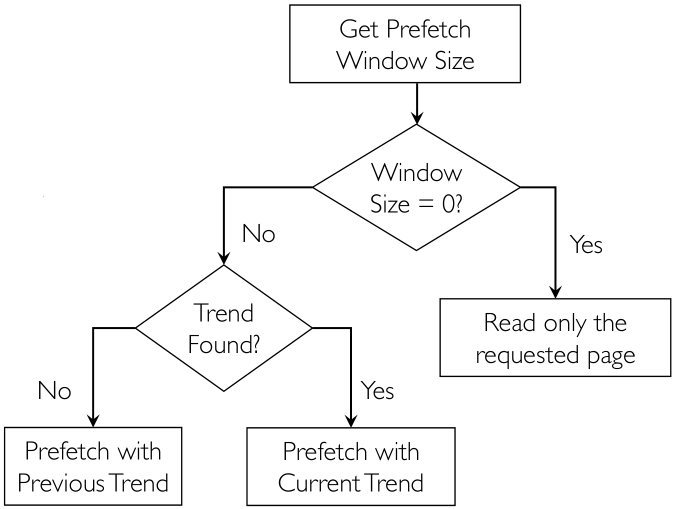
\includegraphics[width=\linewidth]{leap1.png}}
        \caption{Trend-based pefetcher 동작}
        \label{fig:leap1}
    \end{figure}

    Leap의 prefetcher는 hit ratio를 높이기 위해 trend 기반의 prefetching 알고리즘을 사용한다. 구체적으로 각 프로세스들의 원격 페이지에 대한 이전의 접근 history를 바탕으로 해당 프로세스의 페이지 접근 패턴을 추정하게 된다. Prefetch가 활성화 되어있으나 해당 항목들로 패턴을 추정하는데 실패하는 경우에는 이전에 발견했던 trend 패턴을 기반으로 prefetch를 진행한다. 이러한 접근 기법은 기존의 고정적인 prefetch 기법들이 일시적인 특이 패턴에 의해 성능 저하를 보이던 것을 효과적으로 방지해줄 수 있다. 이 내용이 그림 \ref{fig:leap1} 에 정리되어 있다.

    한편으로 history의 size 역시 패턴 결정에 영향을 미치게 된다. 너무 적은 history는 한정된 majority 하에서 패턴을 찾지 못할 가능성을 높인다. 반면에 history가 커지면 연산 부담이 늘어나며, trend가 변화했을 때 따라잡는데 더 오랜 시간을 필요로 하게 된다. Leap는 이 문제를 효과적으로 해결하기 위해, history를 관리하기 위해서도 가변적인 window 크기를 사용한다. 작은 window에서 majority가 존재하는지 먼저 검색하고, 이에 실패했을 때 window를 늘려 재시도하게 된다. 이를 그림 \ref{fig:leap2} 에 나타내었다.

    Prefetch window의 size 역시 중요한 요소이다. 불필요한 prefetch는 temporal locality를 활용하는데 부정적인 영향을 미친다. 하지만 trend가 존재할 때 prefetch의 효과를 보려면 충붕한 prefetch window가 필요하다. 따라서 Leap는 cache hit가 발생했을 때 window를 공격적으로 늘리는 것에 더해, 비록 hit이 발생하지 않았더라도 trend가 존재하는 경우에는 prefetch window를 서서히 늘림으로써 hit가 발생하기를 기대한다. 반대로 trend가 존재하지 않는 경우에는 window를 서서히 줄여나가서 장기간 trend가 존재하지 않을 때 불필요한 prefetch가 진행되는 것을 방지한다. 이러한 컨셉은 이번 프로젝트에 모두 적용되어 있다.

    \subsection{Prefetching in Linux Kernel}

    \begin{figure}[t]
        \centerline{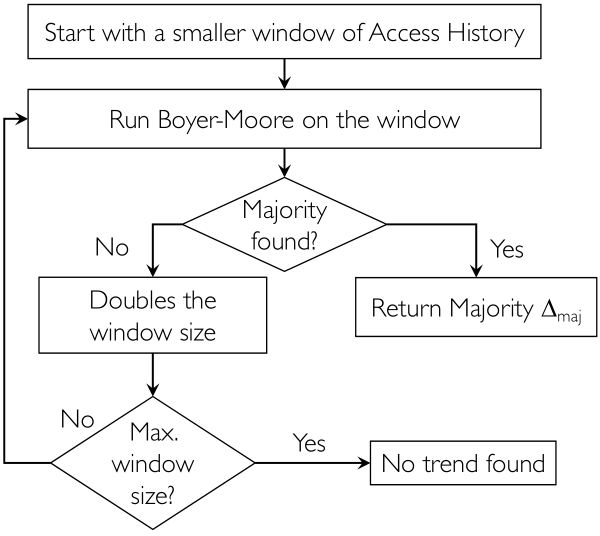
\includegraphics[width=\linewidth]{leap2.png}}
        \caption{Trend detection 동작}
        \label{fig:leap2}
    \end{figure}

    Linux kernel에서 prefetch가 존재하는 항목은 다양하다. 이 연구에서는 해당하는 항목들에 대해 정리하고, 각각에 대해 새로운 prefetch policy를 적용하는 것이 의미있을지 정리하였다.

    먼저 DRAM의 page entry를 CPU cache로 올리는 동작이 존재한다. 이는 모든 컴퓨터 시스템에서 일상적으로 일어나는 동작이며, Linux kernel에는 이 동작의 성능 향상을 목표로 prefetch를 요청하는 구문을 다수 사용하고 있다. 따라서 해당 동작에 대한 변경이 매력적으로 보일 수 있다. 하지만 검토 결과 해당 동작에 대해 Leap의 trend 기반 prefetcher를 적용하기에는 마땅한 위치가 없는 것으로 확인하였다. 구체적으로, 다른 layer에서의 prefetch와 유사하게 주소와 범위를 지정하여 prefetch하는 prefetch\_range() 함수가 존재하지만 주어진 5.4.59 버전을 기준으로 해당 함수에 대한 caller가 없는 것으로 확인하였다. 이전의 history에서도 일부 device driver 등에서만 제한적으로 사용되었으며, 그 외의 prefetch() 호출은 각 code flow에서 다음에 사용할 변수나 객체를 지정하여 prefetch하고 있다. 즉 로우레벨에서 패턴을 임의로 파악하는 것이 아니라 사용자가 직접 이후에 접근할 데이터를 명시적으로 알려주고 있으므로, 이번 연구에서는 개선할 수 있는 내용이 없는 것으로 확인하였다.

    다음으로는 swap 메모리 관리 동작이 있다. Swapping이 동작할 때 전체 시스템의 응답 속도 저하가 매우 크므로, 이를 효과적으로 처리하는 것이 필요하다. 현재 Linux kernel에서는 단순한 readahead 기법을 사용하고 있는 것으로 확인하였다. 이는 page fault가 발생하여 swap 영역을 disk로부터 fetch할 때, 단순히 직전 요청과 연속인 경우 해당 page의 이후 영역 일부를 함께 load하여 이후에 hit되기를 기대하는 것이다. 이러한 단순한 기법도 사용하지 않는 것에 비해 유의미하게 높은 성능을 보여주지만, 순수한 sequential access가 흔치 않으므로 최선의 정책이라고는 할 수 없다 \cite{lwnmmswap}. 특히 이 과정에서 접근하는 프로세스를 구분하지 않으므로 여러 프로세스가 동시에 swap 영역에 접근하는 경우 효과적으로 동작할 수 없다. 따라서 이번 연구에서는 해당 동작에 대해 Leap prefetcher의 trend 탐지 기법을 적용하여 그 성능을 비교하였다.

    추가적으로 파일 접근에 대한 prefetch를 고려할 수 있다. 이는 swap 동작과 일부 유사성이 있으나 구현에 차이가 있으며, 현재의 Linux kernel에는 파일 접근이 sequential read인지 판단하여 readahead 여부를 결정하는 단순한 로직이 포함되어 있다. 이 역시 개선이 가능한 부분이지만, 보다 효과적으로 접근하기 위해서는 해당 파일에 대한 추가적인 특성 역시 함께 고려하여야 한다. 이번 연구에서는 구현에 포함하지 않았으나, 단일 시스템에서의 메모리-디스크 간 prefetch라는 공통점이 있으므로 이 항목에 대한 유용성 역시 간접적으로 평가가 가능하다.

    \subsection{System Implementation}

    연구를 위해 필요한 동작은 세 부분으로 나눌 수 있다: a) trend를 파악하기 위한 history를 갱신하는 동작, b) 해당 history를 바탕으로 trend의 존재를 판단하는 동작, c) trend의 존재 여부에 따라 실제로 prefetch를 수행하는 동작이다. 여기서는 구현과 동작의 효율성을 위해 뒤의 두 동작은 swap in이 필요할 때 함께 수행하였다. history의 경우에는 swap cache에 이미 page가 존재하는 경우 역시 기록하여야 하므로, swap cache에 대한 lookup을 수행하는 위치에서 기록하였다.

    구체적으로 history를 기록하는 log\_swap\_trend() 함수를 구현하고 lookup\_swap\_cache() 에서 호출했으며, trend를 판단하고 prefetch를 수행하는 find\_trend() 함수를 구현해 기존의 swapin\_readahead() 함수에서 호출하도록 작성하였다. 각 함수의 호출 위치와 내용은 Leap 연구에서 공개한 kernel code를 참고하였다. 구현한 상세 코드를 그림 \ref{fig:code} 에 나타내었다.

    \begin{figure*}[p]
        \centerline{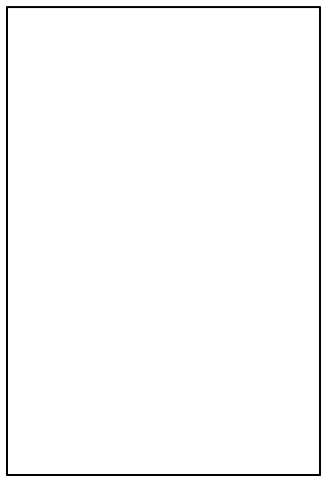
\includegraphics[height=\textheight]{code.png}}
        \caption{구현 코드}
        \label{fig:code}
    \end{figure*}

    \section{Evaluation} \label{sec:evaluation}

    \begin{figure}[t]
        \centerline{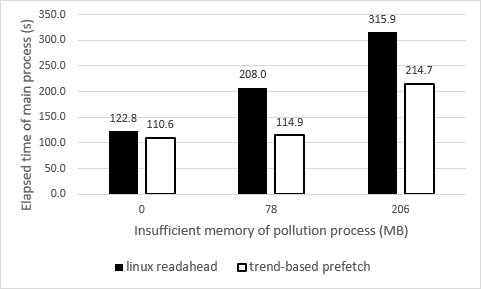
\includegraphics[width=\linewidth]{result.png}}
        \caption{Prefetcher 성능 비교}
        \label{fig:result}
    \end{figure}

    \begin{figure}[t]
        \centerline{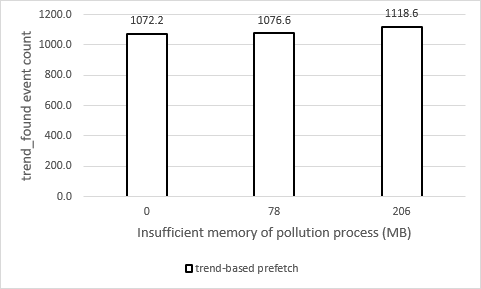
\includegraphics[width=\linewidth]{trend_found.png}}
        \caption{Trend를 찾은 횟수}
        \label{fig:trend_found}
    \end{figure}

    위의 구현에 대한 성능 향상을 평가하기 위한 실험 환경을 구축하였다. 먼저 Intel i5-3230M CPU 2개 코어와 3.8GB RAM이 할당된 Virtualbox 가상머신을 사용하였다. 해당 가상머신에 Ubuntu 20.04.1 LTS를 설치하고 Linux kernel v5.4.59 를 적용하였다. 해당 환경에서 추가적인 수정 없이 default read-ahead를 사용하는 baseline과, 제안 사항이 적용된 trend-based prefetch를 비교하였다.

    단일 노드의 swap 영역에 대한 prefetch 성능을 알아보기 위해, 파이썬 라이브러리인 numpy의 행렬 곱셈 연산 프로그램을 수행하되 사용할 수 있는 메모리 공간을 제한해 swap 공간이 필요하도록 진행하였다. 구체적으로 사용한 행렬 곱셈 연산에 필요한 메모리 공간은 1.7GB였으며, cgroups 명령을 활용하여 해당 프로세스의 메모리 사용량을 1.5GB로 제한하여 주기적으로 swap 이 발생하는 상황을 발생시켰다. 또한 trend-based prefetch의 개선 사항을 자세히 관찰하기 위해 swap cache에 pollution을 유발하는 별도의 process를 병렬적으로 동작시키는 실험을 추가로 진행하였다. 해당 프로세스의 경우 334MB 메모리를 랜덤하게 요청하며 이때 최대 사용량을 가변적으로 제한하였다. 결과 비교를 위해 perf 도구를 활용해 해당 프로세스의 실행 시간을 측정했으며, 또한 kernel 내부에 swapin counter를 설치하여 각 prefetcher의 swap hit 발생 횟수를 측정하였다.

    실험 결과는 그림 \ref{fig:result} 와 같다. Pollution 프로세스에 충분한 메모리가 할당되어 행렬 연산 프로그램만 swap 영역을 사용하는 경우에는 trend-based prefetch가 9.9\% 정도 근소하게 빠른 것으로 나타났다. 이것은 행렬 곱셈이 순수한 sequential access는 아니면서 접근 패턴이 존재하므로, 이 부분에 대해서 우위가 있는 것으로 판단된다. 한편으로 pollution 프로세스와 swawp 영역을 공유하는 상황에서는 두 정책의 성능 차이가 더 크게 보이는 것을 알 수 있다. 구체적으로 최대 78MB의 swap 영역을 요청하는 상황에서 baseline은 성능이 평균 69.4\%나 하락했으나 trend-based prefetch의 경우 성능 감소는 3.9\%로, 랜덤한 접근이 간헐적으로 발생하는 상황에서도 trend가 존재하는 요청에 대해 prefetch를 효과적으로 수행하는 것을 볼 수 있다. Swap 영역이 더 필요한 상황에서도 trend를 추적하여 prefetch할 때 더 높은 성능을 유지할 수 있음을 볼 수 있다.

    이러한 차이의 원인은 각 메모리 사용량 별 trend 검색 횟수를 나타낸 그림 \ref{fig:trend_found} 에서 파악할 수 있다. 실험 결과에 따르면 cache pollution의 존재 여부와 상관 없이 trend-based prefetch가 trend를 확인한 개수는 거의 일정하다. 즉 랜덤한 pollution 접근이 효과적으로 배제되고, trend가 존재하는 행렬 연산 프로세스에 대해서만 prefetch가 효과적으로 수행되고 있음을 보인다.

    이상의 실험 결과를 통해 trend detection의 효과를 확인할 수 있다. 행렬 곱셈 연산 과정에는 분명한 locality가 존재하므로, 단일 프로세스 동작 시에는 기존 Linux kernel의 read-ahead 접근법도 우수한 성능을 보인다. 그러나 swap 영역에 접근하는 다른 프로세스가 존재하는 경우, 각 프로세스로부터의 접근을 구분하지 않는 swap 영역 구현의 특성 상 약간의 충돌로도 baseline은 확연히 낮은 성능을 보여준다. 반면에 trend-based prefetch의 경우에는 작은 프로세스로 인한 성능 저하를 효과적으로 방어하고 있는 것으로 확인할 수 있다.

    \section{Conclusion} \label{sec:conclusion}

    이번 프로젝트에서는 Linux kernel의 swap 영역에 대한 prefetch 성능 개선을 진행하였다. 이를 위해 disaggregated memory를 위한 prefetch 개선 논문인 Leap의 아이디어 일부를 사용하였다. Leap의 trend 판단 알고리즘과 그에 따른 cache pollution 방어가 swap 영역에서도 효과적으로 적용됨을 확인하였다.

    \bibliographystyle{ieeetr}
    \bibliography{citation}

\end{CJK} %
\end{document}

% vim: expandtab wrap
